\begin{frame}[t]{Überblick}

    \begin{spacing}{0.9} \begin{tiny}
            \begin{minipage}{\textwidth}
                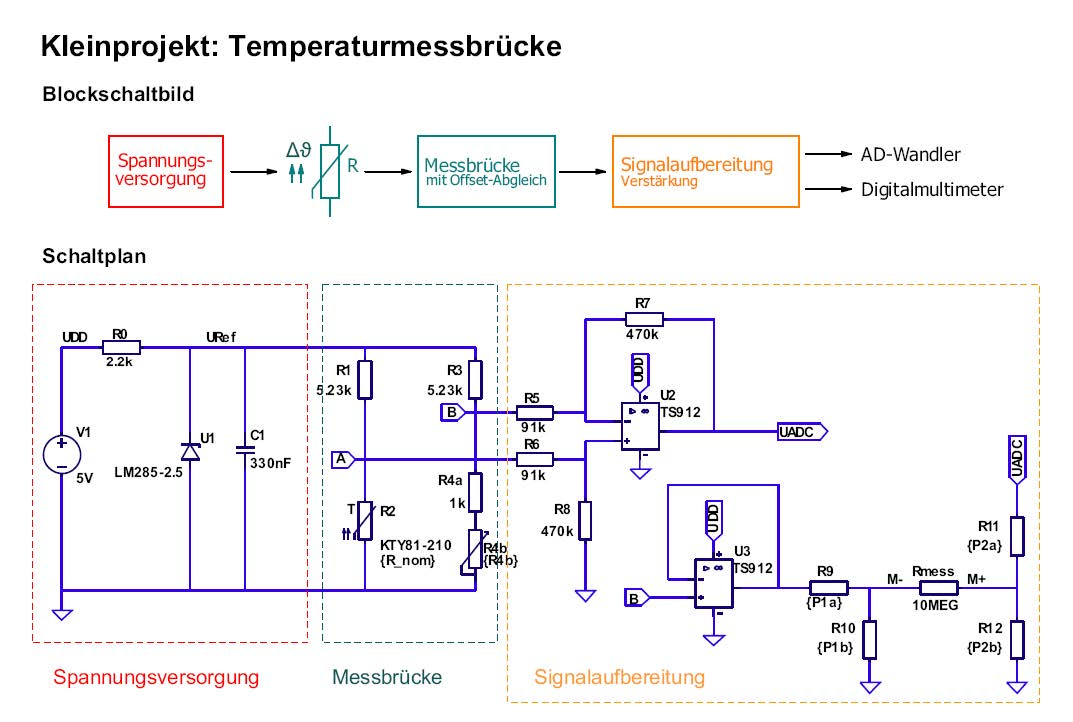
\includegraphics[width=\linewidth]{pictures/projekt_overview.jpg}
            \end{minipage}
        \end{tiny} \end{spacing}

\end{frame}

\begin{frame}[t]{Vorgehenhensweise}

    Zu diesem Zeitpunkt sollten wir alle in der Lage sein einfache Simulationen in DC-,AC-Sweep sowie transient
    durchführen zu können. Sie sollten den Bauteileditor sowie die grundlegenden Schematic-Funktionen (Rotate, Cut, \dots)
    sicher beherrschen.

    Wir werden nun die Bruecke und dir vorgestellten Bestandteile Stück für Stück aufbauen.
    \textbf{Bitte beachtet Folgendes:}

    \begin{enumerate}
        \item Bitte speichert alle Zwischenschritte ab, wir werden Teile später wiederverwenden
        \item Bei Fragen bitten wir euch uns direkt im MS Teams zu benachrichtigen, sodass wir euren
              Fortschritt so gut wie möglich unterstützen können.
    \end{enumerate}
\end{frame}
